\documentclass[12pt]{report}

\newcommand{\titletext}{Semilinaire spectraalanalyse}

\usepackage[dutch]{babel}
\usepackage[nobottomtitles]{titlesec}
\usepackage[bottom]{footmisc}
\usepackage{graphicx}
\usepackage{titleps}
\usepackage{amssymb}
\usepackage{amsmath}
\usepackage{amsthm}
\usepackage{graphicx}
\usepackage{verbatim}
\usepackage{titling}
\usepackage[toc,page]{appendix}
\usepackage{bm}
\usepackage{wrapfig}
\usepackage{subcaption}

\usepackage{fancyhdr}

\pagestyle{fancy}

\renewcommand{\chaptermark}[1]{\markboth{#1}{}}
\renewcommand{\sectionmark}[1]{\markright{#1}}
\fancyhf{}
\fancypagestyle{plain}{%
  \fancyhf{}%
	\rfoot{\fancyplain{}{\nouppercase{\thepage}}}
	\lfoot{\fancyplain{}{Thorvald Dox}}
  \renewcommand{\headrulewidth}{0pt}% Line at the header invisible
  \renewcommand{\footrulewidth}{0.4pt}% Line at the footer visible
}
\lhead{\fancyplain{}{\titletext}}
\rhead{\fancyplain{}{\nouppercase{\leftmark}}}
\rfoot{\fancyplain{}{\nouppercase{\thepage}}}
\lfoot{\fancyplain{}{Thorvald Dox}}
\renewcommand{\footrulewidth}{0.4pt}

\fancyhfoffset[E,O]{0pt}
\date{}
  
\usepackage[margin=1in]{geometry}
\usepackage{float}



\usepackage[super,square,sort]{natbib}
\usepackage{bibentry}
\nobibliography*

%\newcommand{\footcite}[1]{\cite{#1}\let\thefootnote\relax \footnote{\cite{#1} \bibentry{#1}} }
\def\signed #1{{\leavevmode\unskip\nobreak\hfil\penalty50\hskip2em
  \hbox{}\nobreak\hfil(#1)%
  \parfillskip=0pt \finalhyphendemerits=0 \endgraf}}
\newcommand{\rulesep}{\unskip\ \vrule height -1ex\ }

\DeclareMathOperator*{\Odot}{\bigodot}
\allowdisplaybreaks

%\title{Semi-lineair Multiple Endmember mixture spectrum analysis}
\title{\titletext}
\author{Thorvald Dox}

\begin{document}
\begin{titlepage}

\newcommand{\HRule}{\rule{\linewidth}{0.5mm}} % Defines a new command for the horizontal lines, change thickness here

\center % Center everything on the page
 
%----------------------------------------------------------------------------------------
%	HEADING SECTIONS
%----------------------------------------------------------------------------------------

\textsc{\LARGE Universiteit Antwerpen}\\[1.5cm] % Name of your university/college
\textsc{\Large Fysica}\\[0.5cm] % Major heading such as course name
\textsc{\large Masterproef}\\[0.5cm] % Minor heading such as course title

%----------------------------------------------------------------------------------------
%	TITLE SECTION
%----------------------------------------------------------------------------------------

\HRule \\[0.4cm]
{ \Large \bfseries \thetitle}\\[0.4cm] % Title of your document
\HRule \\[1.5cm]
 
%----------------------------------------------------------------------------------------
%	AUTHOR SECTION
%----------------------------------------------------------------------------------------

\begin{minipage}{0.4\textwidth}
\begin{flushleft} \large
\emph{Auteur:}\\
\theauthor % Your name
~\\
~\\
~\\
\end{flushleft}
\end{minipage}
~
\begin{minipage}{0.4\textwidth}
\begin{flushright} \large
\emph{Promotor:} \\
Paul {Scheunders} \\ % Supervisor's Name
\emph{Copromotor:} \\
Rob {Heylen} % Supervisor's Name
\end{flushright}
\end{minipage}\\[5cm]

% If you don't want a supervisor, uncomment the two lines below and remove the section above
%\Large \emph{Author:}\\
%John \textsc{Smith}\\[3cm] % Your name

%----------------------------------------------------------------------------------------
%	DATE SECTION
%----------------------------------------------------------------------------------------

%{\large \today}\\[3cm] % Date, change the \today to a set date if you want to be precise

%----------------------------------------------------------------------------------------
%	LOGO SECTION
%----------------------------------------------------------------------------------------

%
\includegraphics[height=4cm]{remote.png}

\includegraphics[height=4cm]{download.jpg}
\hspace{5 cm}

\includegraphics[height=4cm]{vlabsym.png}
 \\[1cm] % Include a department/university logo - this will require the graphicx package

 
%----------------------------------------------------------------------------------------

\vfill % Fill the rest of the page with whitespace

\end{titlepage}
\tableofcontents


\newpage
\chapter*{Abstract}
\addcontentsline{toc}{chapter}{Abstract (english)}


\newpage
\chapter*{Abstract}
\addcontentsline{toc}{chapter}{Abstract (Nederlands)}



\newpage
\chapter*{Structuur van deze thesis}
\addcontentsline{toc}{chapter}{Structuur van deze thesis}

De inleiding legt uit wat aardopservatie is, welke concepten hiervoor nodig zijn en een aantal toepassingen hiervoor. Dit hoofdstuk is vooral gebaseerd op \textit{Fundamentals of remote sensing\cite{fun}}.

Het eerste hoofdstuk beschrijft ontmengen, en bevat een voorbeeld van een ontmengmethode, namelijk de linaire methode. Ook bevat deze een beschrijving niet-lineaire effecten en variabiliteit. 

In het volgende hoofdstuk worden methodes uit de literatuur beschreven om om te gaan met de problemen beschreven in het vorige hoofdstuk. Enerzijds wordt het multilineair model beschreven, dat gebaseerd is op \textit{A multilinear mixing model for nonlinear spectral unmixing}\cite{mlinmix}. De volgende twee methodes zijn selectiemethoden. Deze methoden zijn ontwikkeld om variabiliteit in rekening te brengen, en staan beschreven in \textit{Hyperspectral unmixing with endmember variability via alternating angle minimization}\cite{mesma}. Deze methoden zijn volledig gekend in de literatuur maar voor deze thesis zijn deze methoden opnieuw berekend en ge\"implementeert. 

Het derde hoofdstuk beschrijft een methode die rekening houd met beide concepten, niet-lineariteit en variabiliteit. Deze is gebaseerd op de methoden beschreven in het vorige hoofdstuk. Dit hoofdstuk bevat ook een numerieke test die gebruik maakt van monte-carlo simulaties.

In het laatste hoofdstuk worden al deze methoden, en een aantal varianten hierop vergeleken aan de hand van een experimentele dataset: de Alina dataset\cite{Alina} en wordt besproken welke methodes en varianten het beste zijn in welke situaties. 
\newpage
\chapter*{Inleiding}
\addcontentsline{toc}{chapter}{Inleiding}

\begin{quotation}
Aardobservatie is de wetenschap van het bepalen van informatie over het aardoppervlak vanop een afstand. Dit wordt gedaan door het meten en vastleggen van gereflecteerde of uitgezonden electromagnetische golven en het verwerken, analyseren en toepassen van deze informatie.
\signed{\textit{Fundamentals of remote sensing\cite{fun} p5}}
\end{quotation}

\begin{wrapfigure}{R}{0.4\textwidth}
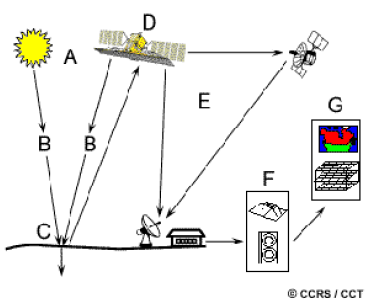
\includegraphics[width=0.4\textwidth]{rs.PNG}
\caption{Aardopservatie \label{fig:rs} Deze afbeelding komt uit \textit{Fundamentals of remote sensing\cite{fun}}}
\end{wrapfigure}


%Het gedetai\"eerde proces verloopt zoals hierna beschreven\cite{fun}, en is te zien in figuur \ref{fig:rs} .

%Een lichtstraal ontstaat aan een zo genaamde lichtbron, wat in de meeste gevallen de zon is. Deze lichtstraal reist door de ruimte en door de atmosfeer, tot deze contact maakt men een materiaal, en hierop een of meerdere keren reflecteert. Daarna reist deze lichtstraal opnieuw door de atmosfeer tot deze contact maakt met een camera op een satelliet. De eigenschappen van deze lichtstraal worden be\"invloed door elk van deze processen.

Aardobservatie begint bij een lichtbron\footnote{In het geval dat men ge\"interesseerd is in het thermisch infrarood spectrum, is er geen lichtbron nodig aangezien materialen op kamertemperatuur van nature dit soort licht uitstralen, ten gevolge van black body radiation.}. Deze lichtbron is vaak de zon, maar dit proces is gelijkaardig voor andere lichtbronnen. De lichtbron zendt een lichtstraal uit, die eerst door de ruimte en vervolgens door de atmosfeer reist, totdat deze contact maakt met een materiaal op het aardoppervlak en hierop een of meermaals reflecteert. Deze reflectie verandert de eigenschappen van de lichtstraal. De gereflecteerde lichtstraal reist opnieuw door de ruimte, totdat deze in contact komt met de detector op een satelliet. Deze detector zet de lichtstraal om in elektrische signalen, die verzonden worden vanaf de satelliet naar het aardoppervlak, waar deze geanalyseerd kunnen worden. Dit volledige proces wordt afgebeeld op figuur \ref{fig:rs}. 



%Elke lichtstraal is een golf in het elektromagnetische spectrum. Deze golf wordt enerzijds bepaald door zijn golflengte, wat de lengte is tussen twee opeenvolgende maxima van de golf, zoals afgebeeld in figuur \ref{fig:golflengte}. Anderzijds wordt de golf bepaald door de intensiteit, wat de grootte is van de piek van de golf. Soms wordt de frequentie van de golf gebruikt om deze te karakteriseren, maar die kan bepaald worden uit de golflengte en de snelheid van het licht. In werkelijkheid is een lichtstraal niet een golf, maar een combinatie van verschillende golven met elk hun golflengte en intensiteit. De bijbehorende intensiteit bij elke golflengte wordt het spectrum genoemd.

\subsubsection{elektromagnetische golven}
Een lichtstraal is een elektromagnetische golf, waarvan een van de belangrijkste eigenschappen voor aardobservatie de golflengte is. Voor een vlakke golf is deze golflengte de afstand tussen twee opeenvolgende cycli, zoals te zien in figuur \ref{fig:rs}. Echter, een lichtstraal is in werkelijkheid bijna nooit een vlakke golf, maar een combinatie van verschillende vlakke golven met verschillende golflengten. De intensiteit van elke vlakke golf voor elke specifieke golflengte wordt het spectrum genoemd. Soms wordt in plaats van golflengte ook frequentie gebruikt, maar deze kan eenvoudig bepaald worden uit de golflengte en de snelheid van het licht.

\subsubsection{hyperspectrale cameras}
Gewone beelden van een camera bevatten drie kleuren, elke passende bij een specifieke golflengte. De keuze voor deze drie kleuren, namelijk rood, groen en blauw, is een gevolg van de beperkingen van het menselijk oog. Dit zijn namelijk de kleuren die een mens kan waarnemen. Om dit beeld digitaal te representeren, moet het beeld opgedeeld worden in kleine, even grote, vierkante elementen, genaamd pixels. Elk van deze pixels bevat voor elke kleur een waarde, die de intensiteit van elke respectievelijke kleur in dit vierkant weergeeft. Hyperspectrale cameras werken in essentie op dezelfde manier, alleen detecteert deze camera niet alleen de hoeveelheid rood, groen en blauw, maar detecteert deze een groot aantal kleuren, genaamd banden. Doordat deze banden meer informatie bevatten dan de banden van een gewone camera, kan hier meer informatie uit gehaald worden. De zon zendt vooral licht uit in het infrarood, zichtbaar licht en ultraviolet en daarom worden er vooral banden gebruikt in dit spectrum, zoals te zien in figuur \ref{fig:specs}.  


\begin{figure}
\center
\begin{subfigure}[b]{0.3\textwidth}
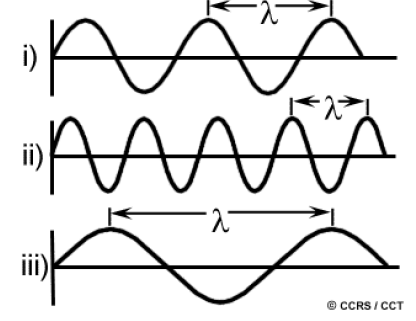
\includegraphics[width=\textwidth]{golflengte.PNG}
\caption{Golven met verschillende golflengten \label{fig:golflengte}}
\end{subfigure} \rulesep
\begin{subfigure}[b]{0.2\textwidth}
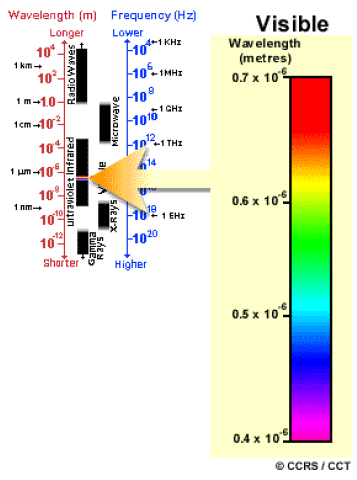
\includegraphics[width=\textwidth]{spec.PNG}
\caption{Het electromagnetische spectrum. \label{fig:spec}}
\end{subfigure}\rulesep
\begin{subfigure}[b]{0.4\textwidth}
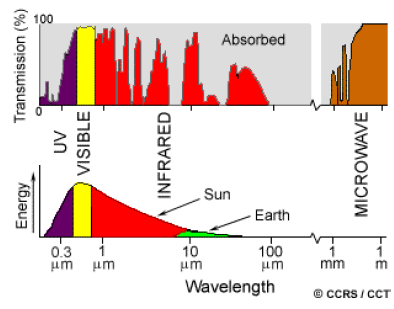
\includegraphics[width=\textwidth]{spec2.PNG}
\caption{Het spectrum van de zon. \label{fig:specs}}
\end{subfigure}
\caption{electromagnetische golven. Deze afbeeldingen komen uit \textit{Fundamentals of remote sensing\cite{fun}}}
\end{figure}


Het doel van spectrale analyse is het bepalen van de hoeveelheden van elk materiaal in een specifieke pixel, gegeven het spectrum van deze pixel. Verschillende methoden hiervoor worden beschreven in deze thesis. 

\section{toepassingen}


Een veelgebruikte toepassing van aardobservatie is het in kaart brengen van landbouwgewassen\cite{fun}. Men kan niet alleen het soort gewas op een akker in kaart brengen, maar ook onder andere de gezondheid en verwachte oogst van verschillende gewassen. In het verleden werd het in kaart brengen van gewassen gedaan door steekproeven te nemen met de hand vanop de grond, maar aardobservatie is nauwkeuriger, goedkoper en kan eenvoudiger gestandaardiseerd worden. Enerzijds is deze informatie nuttig voor de landbouwers zelf, omdat deze aan de hand van de data kunnen bepalen welke gewassen het beste groeien op welke plaats en wanneer er het best gezaaid of geoogst wordt. AAn de andere kant is deze informatie ook nuttig voor overheden en verzekeraars, omdat deze kunnen nagaan welke planten er geplant worden,  voorspellen wat de oogst gaat zijn en bepalen wat de schade is na een droogte of storm. 

Aardobservatie wordt ook toepast in de geologie. Van de aardbodem kan niet alleen het soort gesteente aan de oppervlakte in kaart gebracht worden, maar ook de formatie van deze gesteentes en zelfs de gesteentes liggend onder de aardbodem. Een van de voor de hand liggende toepassingen hiervan is de mijnbouw. Een ander toepassing hiervan is voor het voorspellen van aardbevingen, aardverschuivingen en vulkanisme, wat inhoud dat aardobservatie gebruikt kan worden voor het plannen van wegen, gebouwen en andere structuren. 

  
\begin{figure}
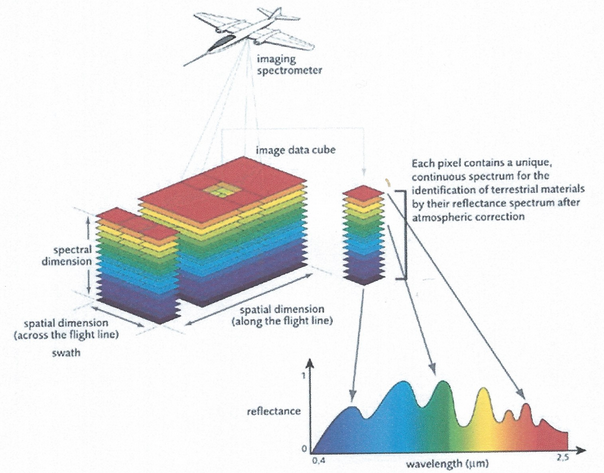
\includegraphics[width=\textwidth]{hyp.PNG}
\caption{Opbouw van een hyperspectraal beeld. Deze afbeelding komt uit \textit{Fundamentals of remote sensing\cite{fun}}}
\end{figure}

\chapter{Ontmengen}



%Het doel van spectrale anaylise is om uit deze hyperspectrale beelden het bepalen welke materialen zich op een specifieke pixel bevinden. Hoewel het belangrijkste toepassing hiervan de aardopservatie is, kan dit evidenterwijs ook gebruikt worden om materialen te analyseren in een laboratorium of voor bijvoorbeeld kwaliteitscontrole in de industrie.

\section{Resolutie}

Een pixel in een hyperspectraal beeld bevat een of meerdere materialen. Een van de belangrijkste oorzaken hiervan is het gevolg van de beperkte resolutie van de camera. De hoeveelheid licht dat op de camera valt is immers beperkt, en moet verdeeld worden over de verschillende pixels en de verschillende banden. Dit betekent dat wanneer de pixels te klein worden, elke pixel te weinig licht krijgt en de signaal ruis verhouding te laag wordt, en aangezien licht bestaat uit fotonen, is er een limiet van de gevoeligheid van de camera. 

De enige methode om de gevoeligheid te verhogen is dus een langere belichtingstijd. Dit zorgt echter voor een vergroting van de ruis en is niet haalbaar voor een satelliet in een baan rond de aarde - zelfs als het praktisch haalbaar was om de resolutie kleiner te maken, ligt het probleem vooral in de fractalische eigenschappen van veel objecten. 

Als we bijvoorbeeld in een bos een zeer grove resolutie gebruiken, vallen er verschillende soorten bomen in een enkele pixel. Als de pixels kleiner worden, kunnen bomen al van elkaar onderscheiden worden, maar de takken van verschillende bomen nog niet. Zelfs als we enkel een blad beschouwen zijn er nog verschillende materialen, aangezien de nerven van het blad een ander materiaal hebben dan de bladmoes. Ook bij mineralen verkrijgen we hetzelfde probleem: een gesteente bevat verschillende mineralen, maar om deze van elkaar te kunnen onderscheiden moet de pixelgrootte al op microscopisch niveau zijn. 

Hierom is het van belang om een spectra van een pixel, dat een combinatie is van de spectra van de verschillende materialen in deze pixel, te kunnen ``ontmengen''. Hierbij zijn we specifiek ge\"interesseerd in de abundantie van elk materiaal: een getal dat het gedeelte van de lichtstralen dat afkomstig is van dat specifiek materiaal weergeeft. Aangezien dit een goede maat is voor de aanwezige hoeveelheid van een bepaald materiaal in een pixel, is dit de belangrijkste parameter waarin we ge\"intereseerd zijn.


\section{spectrale analyse}


Het spectrum van licht kan beschreven worden als een wiskunde functie die een frequentie omzet in een intensiteit. In werkelijkheid bevat een hyperspectraal beeld niet de volledige functie, maar bevat deze tweehonderd waarden in deze functie, de zogenoemde banden. In matlab\citep{MATLAB} zal dit worden opgeslagen als een driedimensionale tensor, waarbij de verschillende assen de x positie, y positie en band van de pixel weergeven. 

In deze thesis zijn we niet ge\"interesseerd in  interpixel-interacties, wat betekent dat het materiaal in een pixel geen invloed heeft op het spectrum van andere pixels, of zeker niet meer invloed tussen naburige pixels dan tussen willekeurige pixels. Daardoor is de exacte structuur van de pixels niet van belang en kan deze worden vervangen door een lijst, dus kan de drie-dimensionale tensor worden omgezet in een matrix, waar de rijen de verschillende pixels zijn en de kolommen de banden.  


%\begin{itemize}
%\item spectra als functies (eigenschappen van licht)
%\item spectra als vector (endmembers) $\rightarrow$ matlab implementatie
%\item mengen van endmembers (abundancies)
%\end{itemize}

\subsection{reflectie}

%Wanneer een lichtstraal invalt op een materiaal reflecteert deze een gedeelte van dit licht. Het nieuwe spectrum van het gereflecteerde licht kan bepaald worden aan de hand van de eigenschappen van het materiaal en het spectrum van het binnenkomende licht. Er kan de benadering gemaakt worden dat de intensiteit voor een gegeven frequentie van het gereflecteerde spectrum alleen afhankelijk is van de intensiteit van het invallende spectrum, en deze daar recht evenredig aan is. In dit geval kan de reflectie beschreven worden als een Hadamard van het spectrum van de inkomende straal en het ``spectrum'' van het materiaal. Dit spectrum is nu geen vector van intensiteiten weer, maar een vector die voor elke frequentie bevat welk deel van de inkomende lichtstraal wordt gereflecteerd. 

Wanneer een lichtstraal invalt op een materiaal reflecteert deze een gedeelte van dit licht en absorbeert de rest. Het spectrum van deze lichtstraal dat gereflecteerd noemt men de reflectantie. Dit is afhankelijk van het materiaal en van de golflengte van het licht. 

In deze thesis worden hiervoor drie aannames gemaakt. Ten eerste heeft de gereflecteerde lichtstraal dezelfde golflengte als het invallende licht. Ten tweede wordt beweerd dat de intensiteit van de gereflecteerde straal recht evenredig is aan de intensiteit van de invallende straal. Ten derde, kan de reflectie van een lichtstraal van een specifieke golflengte niet be\"invloed wordt door licht van een andere frequentie. Deze drie aannames zijn correct volgens de klassieke fysica, maar hier zitten correcties op van kwantummechanische effecten. Deze zullen echter klein genoeg zijn zodat ze als deel van de ruis beschouwd kunnen worden.

De intensiteit van de uitgaande straal kan geschreven worden als volgt:

\begin{equation}
E_{out}(\lambda) = R_\lambda E_{in}(\lambda)
\end{equation}

Dit is een stelsel van vergelijkingen (een vergelijking voor elke waarde van $\lambda$, wat overeenkomt met een band in het spectrum). Zowel de intensiteiten als de reflectieco\"efficienten kunnen samengesteld worden tot een vector, en dan geldt

\begin{equation}
\bm{x} = \bm{R}\odot \bm{y}
\end{equation}

met $\odot$ het Hadamard ofwel elementwijs product. De vector $R$ noemt men de reflectie van het materiaal. Deze neemt in beschouwing dat er meerdere interacties kunnen gebeuren in het materiaal. De reflectie waarbij alleen een enkelvoudige interactie meegenomen is noemt men het albedo.


\subsection{atmosferische correctie}

Wanneer de lichtbron die we beschouwen uniform en genormaliseerd is, is het spectrum van het materiaal gelijk aan het spectrum van het gedetecteerde licht. Alleen is de in werkelijkheid gebruikte lichtbron - meestal is dit de zon - niet uniform. Ook zijn er verschillende effecten die de lichtstraal be\"invloeden\cite{fun} zoals verschuiving, atmosferische verstrooiing, Rayleigh verstrooiing, Mie verstrooiing, nonselectieve verstrooiing, atmosferische absorptie, ozon absorptie, $CO_2$-absorptie en interpixel verstrooiing. De gebruikte datasets in deze thesis zijn al door een algoritme gecorrigeerd voor al deze effecten, en we kunnen deze dus beschouwen als verlicht door een uniforme lichtbron, waarbij de gedetecteerde lichtstraal alleen be\"invloed is door reflecties en Gaussische ruis. 

\section{lineair ontmengen}

Bij lineair ontmengen wordt uitgegaan van het ``lineair mixing model''. In een pixel valt de lichtstraal in op een wel bepaald materiaal, interageert met een enkel materiaal een enkele keer, en valt dan op de detector. Dit betekend dat het spectrum van de teruggekaatste lichtstraal alleen afhangt van de reflectancie van dit materiaal, de endmember genaamd. De totale reflectantie van een pixel die gemeten wordt is echter een gewogen van deze verschillende endmember, waarvan het gewicht van elke endmember bepaald wordt door het gedeelte van de lichtstralen dat op dit materiaal gereflecteerd is. Dit gedeelte wordt de abundantie genoemd. In symbolen geeft dit:


% waarbij uitgegaan wordt dat elke lichtstraal die op een pixel valt enkelvoudig reflecteert en daarna op de detector valt. Het totale spectra op de detector is het gewogen gemiddelde van de spectra van de verschillende endmembers, waarbij het gewicht voor elke endmember de abundantie is van deze endmember. Men krijgt volgende uitdrukking: 


\begin{align}
\bm{x} &= \sum_i a_i \bm{e}_i \label{eq:nq}
\end{align}

Waarbij $\bm{x}$ het gemeten spectrum is, $e_i$ de endmembers en  $a_i$ de abundanties.
Echter, omdat het mixing model slechts een benadering is van de werkelijkheid en omdat op een experimentele meting altijd een vorm van ruis zit, kan het exacte spectrum nooit terug gevonden worden. Er wordt daarom gezocht naar het reconstructiespectrum dat het dichtst ligt bij het werkelijke spectrum. De ruis was verondersteld normaal verdeeld te zijn. Dit is een eenvoudig gevolg van het centrale-limiet theorema, dat zegt dat de som van een groot aantal kansvariabelen normaal verdeeld is. 

Noem $\bm{x}$ het gemeten spectrum, en $\bm{y}$ het reconstructiespectrum, met $\bm{\eta}$ de ruis, dan is

\begin{equation}\label{eq:rec0}
\bm{x} = \bm{y} + \bm{\eta}
\end{equation}

De kans dat $\bm{x}$ gemeten wordt, gegeven dat $\bm{y}$ het werkelijk gemeten spectrum is, is $f(\eta)$, waarbij $f$ de normale verdeling is. Aangezien de normale verdeling alleen afhankelijk is van de kwadratische norm, zijn we ook alleen ge\"intereseerd in de kwadratische norm van de ruis. De normale verdeling is ook groter wanneer deze kwadratische norm kleiner is, dus moet om de kans te maximaliseren de norm van de ruis geminimaliseerd worden. 

Deze norm kan berekend worden gebruik makend van vergelijking \ref{eq:rec0}.

\begin{eqnarray}
\left|\bm{\eta}\right| &= \left|\bm{x} - \bm{y}\right| \label{eq:rec}
\end{eqnarray}

De uitdrukking $\left|\bm{x} - \bm{y}\right|$ noemt men de reconstructie-error. Het is deze uitdrukking dat geminimaliseerd moet worden. 

Het minimaliseren van een uitdrukking om een waarde te vinden noemt men een optimalisatieprobleem, omdat men op zoek is naar de optimale waarden voor de verschillende parameters.

\subsection{minimaliseren van reconstructieerror}
Voor het linair model wordt in dit hoofdstuk er vanuit gegaan dat de endmembers gekend zijn, maar de abundanties en de ruis niet. Als de ruis wordt toegevoegd aan vergelijking \ref{eq:nq} dan geldt:

\begin{align}
\bm{x} &= \sum_i a_i \bm{e}_i + \eta
\end{align}

Het minimaliseren van de reconstructie-error, gebruik makend van vergelijking \ref{eq:rec}:

\begin{align}
\text{argmin}_{a_1 ... a_p} \left| \bm{x} - \sum_{i=1}^p a_i \bm{e}_i\right|^2
\end{align}

Indien de abundanties $a_i$ vrije re\"ele waarden zouden zijn, zou dit minimum eenvoudig berekend kunnen worden, door een projectie te nemen opgespannen door het vlak van de endmembers. Deze projectie kan genomen worden als volgt.

Neem $E = [e_1,e_2,...,e_n]$ een matrix met als kolommen de verschillende endmembers. De projectie op de deelruimte opgespannen door de elementen van $E$ kan gevonden worden aan de hand van het Penrose-invense.

\begin{equation}
\bm{a} = (E^T E)^{-1} E^T \bm{x}
\end{equation}

Doordat de abundanties een gedeelte van de lichtstralen dat op een materiaal botst, zijn er twee extra voorwaarden hierop. Enerzijds moeten de abundanties positief zijn, aangezien men geen negatieve hoeveelheden lichtstralen heeft. Dit noemt de niet-negativiteitsvoorwaarde. Anderzijds kan elke lichtstraal maar op een enkel materiaal botsen, dus is de som van alle delen \'e\'en. Dit noemt de eenheidssomvoorwaarde.  


\subsubsection{niet-negativiteit}

De niet negativiteitsvoorwaarde geeft weer dat de abundanties allemaal positief moeten zijn, of met andere woorden groter moeten zijn dan nul. Dit betekend dat men niet kan projecteren op de deelruimte, maar op een deelverzameling hiervan. Hiervoor kan een aangepast algoritme gebruikt worden, namelijk het ``nonnegative least-squares curve fitting'' of\texttt{lsqnonneg}, maar dit algoritme is veel berekeningsintensiever dan het penrose-inverse algoritme. Later in sectie \ref{sec:select} wordt een alternatieve methode beschreven om met deze voorwaarde om te gaan.

\subsubsection{eenheidssom}

De eenheidssomvoorwaarde geeft weer dat de abundanties moeten sommeren tot \'e\'en. Dit zorgt ervoor dat de mogelijke abundanties geen deelruimte meer opspannen, aangezien het nulpunt geen deel meer is van de deelruimte. Dit kan worden opgelost door een van de endmembers als shadow te beschouwen. Dit houdt in dat het hypervlak verschoven wordt over de vector $e_1$ zodanig dat het nulpunt deel wordt van de hyperruimte en dit terug een deelruimte.

Deze transformatie houdt in dat de matrix $E$ getransplanteerd naar $[e_2-e_1;e_3-e_1;...;e_n-e_1]$ en het gemeten spectrum naar $\bm{x} - e_1$. Na deze transformatie kan het Penrose-inverse algoritme worden toegepast, zodat men de abundanties $a_2,a_3,...,a_n$ krijgt. De laatste abundantie $a_1$ kan gevonden worden door de eenheidssomvoorwaarde te eisen, zodat $a_1 = 1 - \sum{i=2}^{n} a_i$.

\subsection{vrijheidsgraden}

In een optimalisatieprobleem noemt men het aantal re\"ele continue variabelen waarvan een variabele afhankelijk is de vrijheidsgraden. Wanneer het aantal te bepalen vrijheidsgraden groter is dan het aantal gegeven vrijheidsgraden, dan is het probleem ondergedefini\"eerd. Dit houdt in dat er meerdere mogelijke oplossingen voor de vrije parameters zijn waarvoor alle voorwaarden voldaan zijn. Als dit voorkomt, is een gevonden oplossing niet met zekerheid de juiste oplossing, en geeft het model dus verkeerde oplossingen terug, die lijken te voldoen aan het systeem.

Het aantal vrijheidsgraden van het gemeten spectrum is per definitie het aantal banden van de gebruikte sensor. Bij de Avari sensor, welke gebruikt is voor de beelden in dit verslag, is dit $200$. Maar uit dimensionale analyse volgt dat het werkelijke aantal vrijheidsgraden maar rond de $15$ ligt. Als er dus een model gebruikt wordt met meer dan $15$ parameters geeft dit per definitie een goed resultaat, zelfs als dit model totaal niet overeenkomt met de werkelijkheid. Wanneer verschillende modellen vergeleken worden, zal een model met meer vrijheidsgraden een lagere reconstructie-error hebben.  


\section{niet-linaire interacties}

\section{Variabiliteit}\label{sec:select}

\begin{itemize}
\item variabiliteit
\item bibliotheek $\rightarrow$ model
\item pixel-afhankelijke selectie
\end{itemize}


\chapter{Oplossingsmethodes} 

\section{multilineair ontmengen}

Het multilineair model\cite{mlinmix} is een model dat oneindig veel ordes meeneemt, door de interactie van licht met de materialen op het monster te modelleren als een discreet Markov-proces. Deze bevat de volgende stappen, zoals beschreven in \textit{A multilinear mixing model for nonlinear spectral unmixing}\cite{mlinmix}.
\begin{enumerate}
\item De inkomende straal interageert met minstens \'e\'en materiaal in de bron.
\item Na deze interactie heeft het materiaal een kans $P$ om een nieuwe interactie aan te gaan, en een kans $(1-P)$ om dat niet te doen.
\item De kans om een nieuwe interactie aan te gaan met elk nieuw materiaal is evenredig met de abundantie van dat materiaal. Merk op dat aangezien de som van de abundaties \'e\'en is, de waarde van de kans gelijk is aan de abundantie.
\item Wanneer een lichtstraal interageert met een materiaal wordt zijn spectrum gewijzigd, afhankelijk van het albedo van dit materiaal.
\end{enumerate}

De interactie van dit materiaal verloopt als volgt:
\begin{equation}
\bm{x}' = \bm{w} \odot \bm{x}
\end{equation}
waarbij $\bm{x}'$ de uitgaande straal is, $\bm{w}$ het albedo is, $\bm{x}$ de inkomende straal en $\odot$ het Hadamard product, ofwel elementgewijs product wat gedefinieerd is als volgt:
\begin{equation}
\left(\bm{x} \odot \bm{y}\right)_i = x_i.y_i
\end{equation}


\subsection{berekening}

De kans dat een welbepaald pad gevolgd wordt, wordt als volgt genoteerd:

\begin{equation}
\mathcal{P}(i_1,i_2,i_3,...,i_R)
\end{equation}

Bovenstaande uitdrukking geeft de kans dat een lichtstraal respectievelijk reflecteert op materiaal 
$i_1$,$i_2$,$i_3$ en zo voort. $R$ is hier het totale aantal materialen waarop gereflecteerd wordt.

Deze kan aan de hand van het voorgaande Markov-proces berekend worden\cite{mlinmix}. 

\begin{equation}
\mathcal{P}(i_1,i_2,i_3,...,i_R) = P^{R-1} (1-P) \prod_{k=1}^R a_{i_k}
\end{equation}

De uitgaande straal ten gevolge van een specifiek pad is 
$\Odot_{k=1}^R \bm{w}_{i_k}$ dus is de kans op de uitgaande straal vermenigvuldigd met het spectrum:
\begin{equation}
\bm{x}_{(i_1,i_2,i_3,...,i_R)} = P^{R-1} (1-P) \Odot_{k=1}^R \left(a_{i_k} \bm{w}_{i_k}\right)
\end{equation}

Gesommeerd over alle mogelijke paden wordt dit:

\begin{equation}
\bm{x} = \sum_{R=1}^{\infty} \left(\sum_{i_1}^{p} ... \sum_{i_R}^{p}\right)P^{R-1} (1-P) \Odot_{k=1}^R \left(a_{i_k} \bm{w}_{i_k}\right)
\end{equation}

Stel dat de kans dat een lichtstraal nog een keer interageert afhankelijk is van het materiaal. Dit kan voorkomen bij bijvoorbeeld een zandgrond met vegetatie erboven. Een lichtstraal die vertrekt op de grond zal met een grotere waarschijnlijkheid eerst met de vegetatie erboven interageren voor het op de detector terecht komt.

\begin{align}
\mathcal{P}(i_1,i_2,i_3,...,i_R) &= \prod_{k=1}^{R-1}P_{i_k} (1-P_{i_R})\\
&= \prod_{k=1}^{R}P_{i_k} \frac{1-P_{i_R}}{P_{i_R}}
\end{align}


%Nu, laten we de verzameling beschouwen van alle mogelijke paden $(i_1,i_2,i_3,...,i_R)$. Deze kan worden verdeeld in klassen, waarbij elementen in dezelfde klasse worden geplaatst als ze een permutatie zijn van elkaar. Bijvoorbeeld $(1,2,3)$, $(2,1,3)$ en $(3,2,1)$ zitten in dezelfde klassen, maar $(1,2)$,$(1,2,3,4)$ en $(3,4,5)$ zitten allemaal in een verschillende klasse. Als we de $\mathcal{P}$ waarde van elk pad vervangen door het gemiddelde uit zijn klasse, die we $\mathcal{P'}$ zullen noemen, dan blijft de som over de reflectiespectr over alle paden gelijk. Merk op dt dit niet in het algemeen het geval is, maar alleen omdat de paden in eenzelfde klasse hetzelfde reflectiespectrum hebben.
%
%\begin{align}
%\mathcal{P'}(i_1,i_2,i_3,...,i_R) &= \prod_{k=1}^{R}P_{i_k} \frac{1}{R}\sum_{k=1}^{R}\frac{1-P_k}{P_k}
%\end{align}
%
%Veronderstel dat de verschillende $P_i$ waarden bij benadering aan elkaar gelijk zijn. Dit is niet zo een onverwachte eis, aangezien voordien deze waarden exact gelijk werden verondersteld. Met bij benadering gelijk bedoelen we dat $\forall i,j: \frac{P_i}{P_j} \approx 1$ en $\frac{1 - P_i}{1 - P_j} \approx 1$. Dus 0.51 en 0.52 zijn ongeveer gelijk, maar 0.001 en 0.000001 niet, hoewel de laatste twee getallen een veel kleiner verschil hebben. Dan kan het rekenkundig gemiddelde $\sum_{k=1}^{R}\frac{1-P_k}{P_k}$ vervangen worden door het meetkundig gemiddelde $\sqrt[R]{\prod_{k=1}^{R}\frac{1-P_k}{P_k}}
%

De amplitudo van dit pad wordt:

\begin{align}
\bm{x}_{(i_1,i_2,i_3,...,i_R)} &= \prod_{k=1}^{R-1}P_{i_k} (1-P_{i_R}) \Odot_{k=1}^R \left(a_{i_k} \bm{w}_{i_k}\right) \\
&= \Odot_{k=1}^{R-1} \left(P_{i_k}a_{i_k} \bm{w}_{i_k}\right) \odot (1-P_{i_R}) a_{i_R} \bm{w}_{i_R} \\
\bm{x} &= \sum_{R=1}^{\infty} \left(\sum_{i_1}^{p} ... \sum_{i_R}^{p}\right) \Odot_{k=1}^{R-1} \left(P_{i_k}a_{i_k} \bm{w}_{i_k}\right) \odot (1-P_{i_R}) a_{i_R} \bm{w}_{i_R} \\
&= \sum_{i=1}^p (1-P_i) a_{i} \bm{w}_{i} + \sum_{i=1}^p \sum_{j=1}^p (1-P_i) a_{i} \bm{w}_{i} \odot P_j a_{j} \bm{w}_{j} \nonumber\\&+ \sum_{i=1}^p \sum_{j=1}^p \sum_{k=1}^p (1-P_i) a_{i} \bm{w}_{i} \odot P_j a_{j} \bm{w}_{j} \odot P_k a_{k} \bm{w}_{k} \nonumber\\&+ \sum_{i=1}^p \sum_{j=1}^p \sum_{k=1}^p  \sum_{l=1}^p (1-P_i) a_{i} \bm{w}_{i} \odot P_j a_{j} \bm{w}_{j} \odot P_k a_{k} \bm{w}_{k} \odot P_l a_{l} \bm{w}_{l} \nonumber \\& + ... \\
&= \bm{z} + \bm{y}\odot\bm{z} + \bm{y}\odot\bm{y}\odot\bm{z} + ... \\
&= \bm{z} + \bm{y}\odot\bm{x} \\
 &= \frac{\bm{z}}{1-\bm{y}}
\end{align}
waar
\begin{align}
\bm{y} &= \sum_{i=1}^p P_i a_{i} \bm{w}_{i} \\
\bm{z} &= \sum_{i=1}^p (1-P_i) a_{i} \bm{w}_{i} 
\end{align}
zodat
\begin{equation}
\bm{x} = \frac{\sum_{i=1}^p (1-P_i) a_{i} \bm{w}_{i}}{1-\sum_{i=1}^p P_i a_{i} \bm{w}_{i}} \label{eq:Pi}
\end{equation}

\subsection{reflectancy vs albedo}

\subsection{afhankelijke vs onafhankelijke P waarden}



\subsection{Ondergrens van P waarde}

Of dat $P > 0$ moet gebruikt worden als voorwaarde of niet.

\section{MESMA}

\begin{itemize}
\item Ontmengen aan de hand van elke subset
\item Selectie op basis van niet-negativiteitsvoorwaarde
\end{itemize}

\subsection{ontmengingsmethode naar keuze (lineair vs multilineair)}

\section{AAM}

\begin{itemize}
\item concept hoek in hoogdimentonale ruimtes
\item AAM
\end{itemize}

\subsection{implementatie in matlab}


\chapter{Gecombineerde}

\section{Semi-lineair model}

ontkoppeling van Ontmenging in MESMA bij selectie tov ontmenging voor abundancies

\subsection{Theoretische controle dmv monte carlo simulaties}

\section{multilineair AAM}

\chapter{experimentele vergelijking van verschillende methodes}

\section{looptijd en reconstructie-error}

\section{Alina dataset}

\section{Lijst en korte uitleg bij alle methodes}

Elke methode is hiervoor beschreven, maar dit beschrijft kort de verschillen in de methodes en hoe deze geimplementeerd zijn door middel van `schakelaars' in de code. Ook een uitleg bij de weergave van de resultaten. 

\begin{itemize}
\item lineair MESMA
\item semi-lineair MESMA
\item multi-lineair MESMA
\item lineair AAM
\item multilineair AAM
\end{itemize}

$\rightarrow$ Voor de multilineaire modellen wordt ook al dan niet $P> 0$ en $P$ materiaalafhankelijk vergeleken.



\section{Bepreking lineair vs semi-linair}

Verschil voor hoge reflectie (bomen)
$\rightarrow$ semilinair geeft betere resultaten voor dezelfde runtime

\section{Bespreking semi-lineair vs multilineair}

$\rightarrow$ semilineair geeft vergelijkbare resultaten op kortere tijd

\section{Bespreking P-afhankelijkheid}

$\rightarrow$ P-afhankelijkheid geeft vergelijkbare resultaten op gelijke tijd, maar heeft meer vrijheidsgraden

\section{Bespreking P-ondergrens}

verschil voor lage reflectie (asfalt)
$\rightarrow$ Weglaten van ondergrens geeft betere resultaten op gelijke tijd.

\section{Bepreking multilinair AAM vs semilinair model}

$\rightarrow$ zelfde resultaten voor kortere tijd.

\begin{appendices}


\end{appendices}


\begin{flushleft}
\nocite{*}
\bibliography{biblio}{}
\bibliographystyle{plain}
\addcontentsline{toc}{chapter}{Bibliografie}

\end{flushleft}


\end{document}
